\documentclass[12pt]{article}

\usepackage{fullpage}
\usepackage{graphicx, rotating, booktabs} 
\usepackage{times} 
\usepackage{natbib} 
\usepackage{indentfirst} 
\usepackage{setspace}
\usepackage{grffile} 
\usepackage{hyperref}
\usepackage{adjustbox}
\usepackage{amsmath}
\usepackage{siunitx}
\usepackage{multirow}
\setcitestyle{aysep{}}


\singlespace
\title{\textbf{Collective Action or Exchange?: Framing International Cooperation in Alliance Politics}}
\author{Joshua Alley
\footnote{Postdoctoral Research Associate, the University of Virginia.}
}
\date{\today}

\bibliographystyle{apsr}

\begin{document}

\maketitle 

\doublespace 

\begin{abstract}
How do different portrayals of the consequences of international cooperation affect public attitudes towards international institutions? 
There are two general ways to portray international cooperation--- collective action and exchange. 
I explain how using each argument to frame relative defense spending in military alliances affects public opinion towards alliances in large and small treaty partners. 
Although collective action framing increases public support for cooperation in small alliance members, it reduces public willingness to cooperate with allies in larger states. 
Conversely, framing low allied spending as the result of an exchange of protection and influence increases public favorability and support for cooperation in the alliance leader, at the cost of reduced public support in junior members. 
I test these claims with survey experiments on attitudes toward NATO in the United States and Germany. 
My findings provide evidence about how political framing shapes public attitudes towards international cooperation. 
In particular, democratic elites in the leading states of international institutions face a two audience dilemma, as frames  that increase support for cooperation in their country weaken public attitudes in partners. 
\end{abstract}


%\thanks{Thanks to Niels Appeldorn, Alessando Del Ponte, David Fortunato, Matthew Fuhrmann, Nehemiah Geva, Hyeran Jo, Erik Lin-Greenberg and Erik Peterson as well as participants in the 2020 Democratic Statecraft Lab Research incubator and 2019 Oskar Morgenstern Fellowship Colloquium for comments on earlier drafts.}


\newpage 


\section{Introduction}


% Examples to start
In 2016, Barack Obama complained that ``Free riders aggravate me'' and US allies ``have to pay your fair share.'' 
Donald Trump has been more strident in criticizing US allies, especially in the North Atlantic Treaty Organization (NATO). 
In June 2018, Trump wrote to Belgium that: ``it will become increasingly difficult to justify to American citizens why some countries continue failing to meet our shared collective security commitments.''
Other politicians and foreign policy elites dispute this collective portrait of alliances by emphasizing that the United States receives other benefits besides collective security from alliance participation. 
\citet[pg. 129]{RappHooper2020} argues that the US ``alliance system also lowered the cost of US political and military action worldwide.'' 
In a 1999 lecture, John McCain claimed that: ``if we must bear the greatest share of our mutual defense, then our allies must pay as much attention to our concerns, in and out of Europe, as we must to theirs.''\footnote{\url{https://www.k-state.edu/media/newsreleases/landonlect/mccaintext399.html}} 


% introduce the question and make my claim 
This competing rhetoric about alliances raises an important question; how do different portrayals the consequences of international cooperation affect public attitudes towards international institutions? 
In this paper, I identify two general ways to describe the basis of cooperation in international institutions and explain how using these arguments changes public attitudes in different states. 
The first explanation portrays institutional participation as a contribution to some collective good. 
The second explanation emphasizes exchange between states, where cooperation provides differentiated benefits.
Each argument provides a different frame for international cooperation, which may change public opinion \citep{ChongDruckman2007}.  


The divergent processes of the two arguments affect public attitudes towards international cooperation by activating different intuitions and heuristics, which are a function of how individuals understand their state's role in an international institution. 
The public in large states is often concerned with the burdens of maintaining international institutions, while the public in smaller partners emphasizes shared interests and institutional leader legitimacy.
These concerns change how they respond to different frames. 
Relative to a neutral presentation, framing international cooperation in terms of collection action activates conditional cooperation norms and exploitation concerns in the large states that usually lead institutions. 
The same collective action frames increase support for cooperation in small states by indicating that the large state is willing to bear costs of providing goods for all institutional members. 
On the other hand, framing international cooperation as an exchange between states is more likely to increase or maintain public support for international cooperation in leading states by clarifying the benefits of institutional leadership and activating a sense of reciprocity. 
Exchange frames reduce support for cooperation in smaller states by reducing perceptions that the leading states has legitimate authority.  


% note and justify emphasis on alliance politics
While this general argument might apply to institutions and cooperation in multiple issue areas, this paper explores the consequences of framing international cooperation for military alliances. 
I examine alliance politics because discussions of the benefits and burdens of alliance participation clearly show competing frames. 
Alliance politics scholarship is divided between public goods and bargaining models, and foreign policy elites describe alliances in similar ways, as the earlier quotes imply. 
For example, debates over the future of US grand strategy contain two distinct perspectives on alliances, which rely on different arguments. 
Advocates of a restrained US foreign policy often argue that US allies do not contribute enough to their own security, which then increases US defense spending \citep{Preble2009, Posen2014}.
Proponents of continued deep engagement dispute this collective action understanding of alliances and claim that the US gains substantial benefits from alliance participation \citep{BrooksWohlforth2008, BrandsFeaver2017}. 


% specific test
My argument expects that the impact of collective action and exchange frames on public opinion depends on states' roles in international institution. 
I examine the effect of framing international cooperation in large and small institutional members with two survey experiments. 
One study examines attitudes towards NATO in the United States, while the other examines public opinion in the Germany. 
Both studies vary the framing of NATO and relative military spending burdens in the alliance in three ways. 
The first frame uses collective action to describe cooperation in NATO, so under this frame low allied military spending is the result of free-riding in a collective action problem \citep{OlsonZeckhauser1966}.
The second frame explains cooperation among NATO members as an exchange where the US gives protection and gains foreign policy influence \citep{Morrow1991}, so low spending by US allies reflects reciprocity. 
A neutral frame with no frame or information about allied spending is the reference category for the two competing frames and information about military spending.


% I find that...
In an initial test of the argument on Mechanical Turk, I find mixed support for the argument.
In the United States, exchange framing increases favorability towards NATO, and collective action may reduce support for military intervention, but the effects are fairly weak. 
In Germany... 


% Detail contribution: start with academic models
The argument and findings have four general implications.
First, I present indirect evidence whether regular condemnations of allied ``free-riding,'' most recently by Donald Trump, could affect public attitudes toward international cooperation, which adds to the rich literature on political rhetoric and public opinion in the United States. 
It also highlights that the collective action logic behind some of these complaints bolsters support for NATO outside the United States.  
Using different explanations to frame international cooperation is a novel mechanism for understanding individual attitudes towards international institutions and cooperation. 
Existing scholarship on international economic cooperation, especially trade, uses economic interests e.g. \citep{Rogowski1987, MaydaRodrik2005} or perceptions of the costs and benefits \citep{Hainmueller2006, MansfieldMutz2009, RhoTomz2017} to explain public attitudes. 
\citet{Edwards2009} uses a mix of economic and ideological factors to predict support for the IMF, World Bank and WTO in developing countries and \citet{BearceScott2019} argue that individual economic concerns affect attitudes toward international institutions. 
These studies and other surveys on public attitudes towards international institutions use standard survey questions \citep{KayaWalker2014, DellmuthTallberg2015}.
Neutral questions avoid leading respondents, but they do not correspond to how political actors discuss international institutions, which is a key source of public information, as the media partially transmits elite foreign policy frames \citep{BaumPotter2008}. 
Politicians, the media and other foreign policy elites frame international cooperation with different explanations to advance their goals, so common sources of information about international institutions are more slanted than the typical survey question.  


% Taking public goods and framing out of the lab
Second, the findings broaden our understanding of framing effects and may apply to cooperation beyond alliance politics and international relations.  
Most frames in survey experiments on international security examine public support for using force, but this experiment addresses interstate security cooperation. 
More generally, a vast literature examines how individuals view and contribute to collective action in laboratory settings e.g. \citep{Ostrometal1992, GachterFehr1999, Houseretal2008, Aimoneetal2013}. 
Framing is a common and powerful manipulation in these laboratory experiments, and I show how it affects attitudes towards cooperation outside the lab. 


Third, I identify a crucial consequence of ideas in international relations. 
As \citet[pg. 50]{BoettkeAligica2009} write, ``Ideas set into motion actions, ideas give solutions but they also generate new problems and challenges.''
Existing research shows that ideas shape how leaders understand the costs and benefits of different policies \citep{Morrison2012, Morrison2016} and can give leaders a means of justifying their preferred policy \citep{Parsons2002}.
The same is true of the public--- exposure to different academic and popular explanations of the consequences of international cooperation affects public attitudes.


Last, this paper contributes to knowledge of the domestic politics of alliances \citep{Lobell2004, Mattes2012a}.
Public attitudes towards international institutions are important, especially in democracies, where public support can restrict leaders' policy choices \citep{Putnam1988, Fearon1998, LevenduskyHorowitz2012, Williams2013, Levyetal2015}. 
Because public attitudes shape the willingness of leaders to use force \citep{Tomzetal2020} and alliances are formal efforts to establish credible commitments of military intervention \citep{Morrow2000}, public perceptions of allies affect the credibility of the alliance. 
If elites use frames that raise the fear of exploitation by allies or weaken public support in other countries, subsequent changes in support for fighting alongside allies may undermine the alliance itself.  


This paper proceeds as follows. 
First, I explain how framing international cooperation in terms of collective action or exchange affects public attitudes towards international alliances. 
Then, I describe the design and results from survey experiments attitudes towards NATO in the United States and United Kingdom that test six predictions from that argument. 
Last, I offer some concluding thoughts for scholars and policymakers. 



\section{Argument}



% Outline the argument
The argument proceeds as follows.  
First, I explain why framing could affect public attitudes towards cooperation.
Following that, I detail collective action and exchange frames of international cooperation. 
I then describe cooperation in alliances and competing explanations of why US allies spend a smaller share of their resources on the military.  
Then I describe the consequences of collective action and exchange framing for public support of alliances. 
I also explain how foreign policy information and partisanship may modify the effect of framing. 


What produces different frames for international cooperation? 
Frames are ways actors present information, and they often employ an explanation of how the world works. % expand definition if needed
Collective action or exchange reciprocity are two likely frames for international cooperation.
Under collective action group members all contribute to some common or collective good. 
Exchange reciprocity portrays cooperation in terms of trading different goods, so group members receive differentiated benefits, rather than a single collective good. 


Framing international cooperation, is a political act.  
Framing is political because frames define problems and corresponding solutions.\footnote{Solving a collective action problem requires careful attention to institutional rules \citep{Ostrom1990} or judicious use of select incentives \citep{Olson1972, Hardin1982}.
On the other hand, cooperation through exchange requires attention to other contracting issues \citep{Williamson1985}.}  
After framing cooperation, political elites can then advocate policies that match their interests and agenda.
Any solution or policy change, including maintaining the status quo, has distributional consequences. 
Sanctioning institutional participants for free-riding in the face of an ostensible collective action problem will benefit some actors more than others, for example.


% Discuss why framing can work
Adopting different frames for international cooperation affects public attitudes for two reasons. 
First, lab experiments provide ample evidence that how researchers frame cooperative games affects affects individual attitudes and behavior. 
Scholars have explored a wide range of frames for a common public goods game, which they usually present as generic investment or decision-making. 
In the voluntary contribution mechanism game, individuals can invest experimental tokens in public or private accounts, and the whole group benefits from public investments. 
Maximal investment in the public good is the Pareto optimal choice, but individuals have incentives to defect, which creates a collective action problem.
Framing impacts cooperative behavior in the lab through different subjective understandings of the underlying game \citep{Cookson2000, CartwrightRamalingam2019}. 
Changing the frame alters the weight people give particular values while forming opinions \citep{ChongDruckman2007} and beliefs about other players \citep{Dufwenbergetal2011}.
The power of framing in the lab should apply elsewhere, because the lab and field have a common psychological base. 


Second, the public has limited information about international affairs and cooperation.
Limited information gives frames more power \citep{Druckman2001}, as it makes public opinions more malleable. 
Different subjective understandings from frames in the lab occur when participants do not grasp the ``true'' underlying game. 
This gives researchers and other participants freedom to frame.
Thus, political frames of international cooperation depend on limited information and can affect how people view cooperation.  


% Framing int'l cooperation has two audiences
Elite frames and rhetoric about international cooperation have international and domestic audiences. 
When elites in the leading members of international institutions discuss cooperation, their discourse reaches the public in their state, as well as elites and the public in other states. 
Thus public framing is part of a two-level game, where elites justify international institutions and cooperation to foreign and domestic audiences \citep{Putnam1988}.
To sustain international cooperation, elites in leading states must balance the concerns of their public and foreign audiences. 
In institutions where the public has foreign policy influence, public support at home or abroad can undermine cooperation. 
This balance creates a dilemma in alliance politics, as frames collective action and exchange frames have competing effects on the public in leading and junior members of international institutions.\footnote{Considering public responses creates a clear scope condition on the argument, as it applies best to cooperation between democracies. Alliances between autocracies and democracies or between autocracies lack domestic and foreign public audiences.}


\subsection{Framing Alliance Politics}


% Alliance politics here
I explore the consequences of framing defense spending in alliances because frames match real-world debates and could change public attitudes.  
Different frames are possible in alliance politics because elites present cooperation in competing ways and the public has little knowledge of alliance politics. 
Exchange and collective action models offer different ways to explain cooperation in alliances and military expenditures by alliance members.
Therefore, each argument provides a different frame for alliance politics and differences in military spending between large and small alliance members. 


\citet{OlsonZeckhauser1966} and \citet{SandlerHartley2001} offer two well-known models where alliances produce full or partial public goods.
In this model, all alliance members receive security and contribute to security through their military spending. 
Public goods models then argue that lower defense spending by small alliance members reflect a collective action problem, where small states free-ride on larger partners. 


Exchange-based models argue that alliances, especially asymmetric treaties between large and small states, can reflect trades between states with heterogeneous goals. 
Alliance members exchange different benefits as junior partners gain security and senior partners gain influence \citep{Morrow1991}. 
Thus, small states may lower defense spending because they gave up foreign policy autonomy in exchange for protection.
Rather than contribute to collective security alliance members receive different goods through treaty participation. 


The public also has limited information about alliances, so alliance politics meets a key criterion for frames to affect public attitudes. 
Alliances can be salient in domestic politics when they engage promises of military support, but the public has limited information about alliances otherwise. 
Models of alliance politics are disputed by elites and unknown to the public, so different frames are possible and could alter subjective beliefs.
Inasmuch as the public does not have ready-made frameworks to conceptualize cooperation in alliances, they will rely on heuristics and intuitions to parse information from elite cues \citep{BaumPotter2008}.\footnote{I will examine whether individuals with more foreign policy knowledge are less sensitive to framing, as \citet{Druckman2001} claims.} 


% Introduce a neutal baseline
I compare the collective action and exchange frames to a neutral portrayal of allied defense spending. 
A neutral presentation with no explanation of the causes and consequence of international cooperation contains no framing elements. 
Neutral framing thus approximates baseline attitudes. 
Frames add information about the causes and consequences of international cooperation. 
In military alliances, relative military spending is a salient and observable consequence of cooperation that is closely tied to the two frames. 
Larger alliance members often spend a larger share of their resources on the military, which could reflect free-riding or efforts to extend influence by protecting smaller states. 


How exchange and collective action frames impact public attitudes towards alliances depends on the place of their state. 
The public in junior alliance members has different concerns than the public in the alliance leader. 
In large states, the public is interested in whether the costs of alliances provide adequate returns. 
The public in smaller states is more concerned with whether the alliance leader accounts for their concerns and interests. 
Thus, collective action and exchange frames will have different effects. 
I start by describing the impact of these frames on the public in larger states. 


\subsubsection{Leading Alliance Members}


% public concerns in large states: is protecting allies worth it? 
The public in large states is interested in whether protecting allies is worthwhile, or more generally if the benefits of international cooperation outweigh the perceived costs. 
Therefore, the perceived benefits of cooperation and the role of other states are essential to understanding public attitudes. 
If the public in the leading alliance members knows that allies have lower military spending than their state, the explanation for those spending decisions is crucial.  


% discuss the consequences of adopting a collective action frame
% Mechanism one here
Relative to a neutral frame, I expect that using collective action to describe relative military spending burdens will decrease support for alliance cooperation among the public in large states. 
There are two mechanisms behind this relationship.
First, collective action frames raise fears of exploitation. 
Individuals do not want to be taken advantage of. 
Lab experiments on collective action corroborate the intuition that individuals dislike receiving a sucker's payoff. 
Cooperative individuals are often willing to punish free-riders, even at substantial cost to themselves \citep{FehrGatcher2000, Seftonetal2007}.\footnote{Such sanctions can promote cooperation \citep{Guererketal2006}, but punishment is not always effective \citep{Houseretal2008} or efficient \citep{Pageetal2005, Seftonetal2007, Randetal2009}.}


% Mechanism two here
Second, collective action framing of low allied defense spending reduces public support for alliances through conditional cooperation norms. 
Substantial evidence from public goods experiments suggests individuals are willing to cooperate so long as others also cooperate \citep{Chaudhuri2011}.
Defection in the lab often generates social disapproval \citep{GachterFehr1999, Cubittetal2011a}, and may present a moral dilemma as individuals fear violating norms \citep{Nielsenetal2014}. 
When other players do not contribute to the collective good, individuals are less willing to cooperate.\footnote{Beliefs about cooperation and cooperative behavior in the lab depend on other players' contributions \citep{FischbacherGachter2010}.}


% discuss the consequences of employing an exchange frame
Using exchange to explain allied military spending has different consequences for public attitudes in the leading alliance member. 
Explaining allied military spending through a mutually beneficial trade is less likely to raise a sense of exploitation, because low allied defense spending is no longer presented as an inadequate contribution to collective security. 
It also matches a different underlying psychological tendency. 
People are used to exchanging different favors.
This willingness to engage in exchange reciprocity is present even in impersonal laboratory experiments \citep{McCabeetal1996}. 
Individuals understand that cooperation can yield a larger total prize, which facilitates reciprocity and social exchange \citep{Hoffmanetal1998}. 


With exchange, both sides benefit from cooperation, albeit in different ways. 
Both parties to an exchange gain something, but their gains need not be equivalent or proportionate to make trading worthwhile. 
Thus, if individuals believe that they or their country benefits from cooperation, even if partners do not behave in the same way, they will be more likely to support cooperation. 
For example, explaining the consequences of protectionism increases support for trade liberalization by individuals who might benefit \citep{RhoTomz2017}.\footnote{Of course, if individuals believe an exchange is unfair, they will not support it.}


% Relevant attitudes: favorability, withdrawal, and military support
There are three crucial attitudes in the alliance leader's public.
The first is general favorability towards alliance participation. 
The second is a commonly discussed policy response to low allied spending--- withdrawal from the alliance. 
If the public is willing to support withdrawal, they are less likely to penalize leaders who take such steps. 
The third and final attitude is support for military intervention, as public support for intervention helps leading alliance members make credible commitments. 


% state the hypotheses
Collective action frames will decrease favorability, increase support for withdrawal, and reduce support for military intervention among the public in an alliance leader. 
On the other hand, exchange framing of allied military spending will increase individual favorability towards alliances, reduce support for withdrawal and increase support for military intervention in large states, relative to a neutral frame. 
Under exchange, the understanding that cooperation produces heterogeneous benefits and the alliance leader gains influence through protecting allies, means that low allied military spending is not a barrier to public approval. 
Exchange and collective action frames will have the opposite effect on the public in smaller alliance members, however. 


\subsubsection{Junior Alliance Members} 


The public in junior alliance members faces different considerations.
They are more sensitive to giving up their interests and autonomy under an alliance and concerned with the legitimacy of institutional leaders. 
Unlike the public in the alliance leader, who may not perceive the influence their state has over alliance partners without  an explicit exchange frame, the public in small states is more likely to understand alliance leader influence over their foreign policy freedom. 
Whether the alliance leader is sensitive to the foreign policy concerns of small states is a crucial source of legitimacy for the public in junior partners. 
As a result, collective action and exchange frames therefore active different mechanisms. 


Collective action framing increases support for alliance cooperation in small states by activating positive conditional cooperation norms and increasing the legitimacy of the alliance with the public. 
Under a collective action frame, large and small alliance members reap the same benefits from alliance participation, and the leader makes a disproportionate contribution to security. 
Such costly cooperative behavior by the leader may increase favorability towards the alliance and support for additional cooperation. 


In addition to activating conditional cooperation considerations, collective action framing increases the legitimacy of the alliance in junior partners. 
The willingness of the large state to bear a disproportionate share of the burden of providing security generates perceptions of benevolent leadership.
This in turn increases perceptions that the alliance leader has legitimate authority, as a collective action frame emphasizes large benefits for the group that favor smaller states.
\citet{Lake2013} identifies this distribution of benefits as a crucial source of legitimacy in hierarchical relationships.
To put it differently, if the leader bears the costs of providing security for the whole alliance, it signals a commitment to restrained leadership that is in the interest of junior partners. 


% exchange frames have the opposite effect
Exchange frames are more likely to reduce support for alliance cooperation in junior alliance participants, even if they accurately capture limits on foreign policy freedom. 
Exchange frames clarify that junior alliance partners give up some foreign policy freedom in exchange for protection. 
This turn generates doubt over whether the alliance leader has the best interests of junior partners in mind, or is purely self-interested. 
Exchange casts the alliance relationship as a transaction and raises fear that the larger partner will or is trampling on the interests of junior partners. 


% further explanation
No states have perfectly congruent foreign policy interests, even alliance members. 
For example, NATO members differ in their ``Atlanticist'' orientation \citep{BeckerMalesky2017}. 
Thus, small alliance members do lose the freedom to pursue some foreign policy goals in an alliance. 
The public in these states may find such exchanges distasteful. 
Making an implicit understanding about protection and foreign policy influence explicit through an exchange frame will not sit well with the public.\footnote{A possible extension of this project could measure implicit views of NATO in multiple countries and examine whether a more collective action understanding of alliances is positively correlated with NATO favorability.}


% outcomes/key attitudes: favorability, support for increasing spending, support for intervention
This argument makes predictions about three similar attitudes in junior alliance members--- favorability towards alliance cooperation, policy responses to military spending concerns, and support for military intervention. 
I expect that collective action framing will increase favorability towards alliances, but exchange framing will decrease favorability in junior alliance partners. 
To assess policy change, I consider whether the public in small states is willing to increase their defense spending, and expect more support for higher military spending under collective action frames, but less support under an exchange frame.
Under exchange, protection from external threat for junior members does not depend on their military spending. 
Last, I expect that collective action frames will increase support for intervention to support allies in war, while exchange frames will decrease support for intervention. 
Under collective action frames, intervention supports the security of the whole alliance, but this general cooperative relationship is absent under exchange. 


% dilemma- frames that play well abroad are less effective at home
The contradictory responses of the public in the alliance leader and junior states creates a dilemma for elites in the alliance leader. 
If they emphasize collective action frames, they shore up support abroad at the cost of support at home. 
On the other hand, exchange frames bolster public support for alliance cooperation at home, while weakening it abroad. 
To examine the extent of this dilemma, I use the general argument to make testable predictions about attitudes towards NATO in the United States and Germany. 


\subsubsection{Hypotheses}


I focus on public opinion towards the North Atlantic Treaty Organization (NATO) for three reasons. 
First, collective action and exchange frames are already present in discussions about military spending by NATO members, which draw on the broader theoretical division in models of alliance politics.
For example, \citet{Lanoszka2015} asserts that NATO reflects a bargain where American protection is contingent on foreign policy support and nuclear non-proliferation, so low allied spending is not free-riding. 
Other researchers claim that low allied spending is the result of free-riding, however e.g.\citep{OlsonZeckhauser1966, PluemperNeumayer2015, KimSandler2019}.
Second, when the public in the United States and Germany thinks of alliances, NATO is the most likely subject, so considering attitudes towards NATO has less risk of confounding from implicit associations. 
Third, studying NATO allows me to compare the theoretical frames with standard survey results.


% Focus on US and Germany
Why examine the United States and Germany? 
The United States is the alliance leader in NATO, as it is the most capable and influential member by far. 
I examine public attitudes towards NATO in Germany because Germany has a wide range of public opinions towards NATO. 
During the Cold War, Germany received substantial security benefits from NATO membership. 
However, modern German opinion towards NATO is more mixed, due to reduced external threat and regional differences between East and West Germany.
Residents of the former East Germany have less connection with US troops and bases. 
Although Anglophone countries like the United Kingdom and Canada are another obvious survey domain, these states have distinct, ``special'' security ties with the US, so opinions there may be less representative of attitudes in junior NATO members. 
Studying Germany also allows me to examine the effects of framing on a key European NATO member. 


I now articulate six hypotheses- three for each study. 
First, collective action and exchange frames should have different effects on favorability towards NATO in the United States. 
Collective action framing of allied military spending will decrease favorability, but exchange framing should increase favorability. 


% Prediction 1
\begin{quote}
\textsc{Hypothesis 1}: Compared to the neutral frame, US respondents will have less favorable views of NATO in the collective action frame, and more favorable views in the exchange frame.  
\end{quote}

Second, framing will affect support for leaving NATO in response to allied military spending. 
Under collective action, more respondents will favor leaving the NATO treaty. 
But low spending should be perceived as less problematic in the exchange frame, which will make respondents less likely to support leaving the alliance entirely. 


% Prediction 2
\begin{quote}
\textsc{Hypothesis 2}: Compared to the neutral frame, more US respondents will support leaving NATO in response to low allied military spending in the collective action frame, while fewer respondents will support leaving NATO in the exchange frame.
\end{quote}


Finally, framing allied military spending will change support for military intervention on behalf of NATO members. 
Given conditional cooperation norms and concern with exploitation, collective action framing will reduce public support for intervention. 
Exchange framing should increase support for intervention, however. 


% Prediction 3
\begin{quote}
\textsc{Hypothesis 3}: Compared to the neutral frame, fewer US respondents will support military intervention to defend a NATO member in the collective action frame, and more respondents will support intervention in the exchange frame. 
\end{quote} 


As noted above, collective action and exchange frames will have the opposite effect on the public in junior alliance members. 
That leads to the following hypotheses about public attitudes towards NATO in the Germany.  
First, collective action framing of military spending in NATO will increase favorability, and exchange framing will decrease favorability. 


% Prediction 4
\begin{quote}
\textsc{Hypothesis 4}: Compared to the neutral frame, German respondents will have more favorable views of NATO in the collective action frame, and less favorable views in the exchange frame.  
\end{quote}


The two frames will also impact willingness to increase military spending. 
Under collective action, more respondents will favor higher spending. 
But exchange framing will make respondents less likely to favor greater defense spending, as security from the alliance does not depend on small states' spending. 


% Prediction 5
\begin{quote}
\textsc{Hypothesis 5}: Compared to the neutral frame, more German respondents will support increased military spending in the collective action frame, and fewer respondents will support higher spending in the exchange frame.
\end{quote}


Finally, framing allied military spending will change support for military intervention on behalf of NATO members. 
Collective action framing will increase public support for intervention in junior alliance partners. 
Exchange framing should decrease support for intervention, however. 


% Prediction 2
\begin{quote}
\textsc{Hypothesis 6}: Compared to the neutral frame, more German respondents will support military intervention to defend a NATO member in the collective action frame, and fewer respondents will support intervention in the exchange frame. 
\end{quote} 



In both studies, the first response question deals with attitudes towards NATO, while the second and third questions consider support for particular policies. 
A priori, I expect that framing will have a larger effect on favorability towards NATO than attitudes towards policy. 
Attitude changes have fewer cost and countervailing considerations than policy changes. 


These hypotheses have two further implications. 
First, there should be clear differences in attitudes between the exchange and collective action frames. 
Second, if my argument is correct, framing works because the public has limited foreign policy information. 
Therefore, respondents with high foreign policy information may be less sensitive to framing \citep{Druckman2001}. 


%discuss partisanship and pandering
Partisanship may also condition how individuals respond to the two frames. 
Republicans tend are often skeptical of international institutions and NATO, while Democrats have more favorable views.
By attributing the alliance frames to the a non-partisan think tank, I hope to avoid partisan cues, but information about alliances may reinforce existing views. 
For example, Republican skeptics of NATO may be more sensitive to exploitation concerns in the collective action frame, while Democratic support may be further bolstered by the exchange frame. 
Again, I test this conditional relationship later in the analysis. 


Although my argument asserts that the public responds to elite cues and rhetoric, elites might instead pander to existing public attitudes.\footnote{\url{https://fivethirtyeight.com/features/is-trump-fueling-republicans-concerns-about-nato-or-echoing-them/}}
If elite rhetoric on alliances is mostly pandering, then individuals could discount the frames entirely and retain their original alliance attitudes.
This implies stable attitudes toward alliances that elites can pander to.  
Elite pandering to public attitudes towards international cooperation is unlikely for three reasons, however. 
First, \citet{Canes-Wrone2006} finds that Presidents rarely pander to the public unless they already agree with public preferences, and are more likely to match public opinion on everyday issues for voters \citep{Canes-WroneSchotts2004}.  
Second, public attitudes are not stable and exogenous to elite messaging in general \citep{Druckman2014} and low foreign policy information in the public should accentuate the importance of framing.
Third, foreign policy is not the primary concern of many voters, so elite foreign policy views and rhetoric can diverge from public attitudes with limited fear of political repercussions \citep{BusbyMonten2012}. 


Even if pandering is unlikely, this experiment may offer a way to differentiate between the pandering and elite cues models of public opinion towards alliances. 
If the frames have little effect, that may imply that public opinion is unresponsive to elite cues. 
A null effect of the treatments does not imply that elite rhetoric towards alliances panders to the public, however. 
Elites may have their own foreign policy views, or engage in rhetoric primarily for international audiences. 


In the next section, I describe the design of the survey experiment. 
I use the same treatment vignettes for the US and German samples. 
The two studies only differ in one question about policy change in response to military spending differences. 


\section{Experimental Design}


In the survey experiment I vary descriptions of NATO and relative military spending among alliance members. 
Each description provides a distinct frame, either neutral, collective action, or exchange. 
The design draws on a growing literature linking political behavior and international relations \citep{Hafner-Burtonetal2017} and offers a clean test of whether changes in framing alter public attitudes towards alliances.


The treatment in the experiment is a short vignette on NATO. 
A neutral control vignette introduces NATO and mention that allies spend a smaller share of their resources on defense than the United States. 
In the second vignette, my description of NATO explains allied military spending with collective action language that highlights disproportionate US contributions.\footnote{I do not use the words ``free-riding,'' because this explicit label could activate extant preferences, specifically general aversion to free-riding.} 
The third vignette emphasizes exchange between the United States and its allies to explain allied defense spending. 


% Justify emphasis on observed case, not hypothetical scenario 
The survey focuses on NATO rather than a hypothetical alliance for three reasons. 
First, explicitly discussing NATO avoids confounding effects, which are a potential threat to inference in survey experiments, especially those with a short vignette \citep{KrepsRoblin2019}. 
Confounding occurs when respondents impute characteristics to the survey situation, and NATO is the most likely confounder. 
When the public thinks about alliances, NATO is the most likely subject because it is the best-known international alliance.
Second, debates about relative military spending are well established in NATO. 
As a result, the experiment approximates the effects of ongoing policy debates on public attitudes. 
Last, studying NATO facilitates comparisons with earlier surveys.
 

Because framing has political implications, who frames NATO and allied military spending matters. 
In the vignettes below, I attribute the information about NATO to an unnamed expert with the Council on Foreign Relations, a non-partisan think tank in the United States. 
Given extensive partisan polarization, using a partisan political elite for the alliance cue could wash out the effects of the collective action or exchange information \citep{Druckmanetal2013}. 
I now summarize the three vignettes, with the differences in italics. 
 
 
\begin{enumerate}

\item \textbf{Neutral}: The North Atlantic Treaty Organization (NATO) is a military alliance where members promise to support one another in war. According to an expert at the Council on Foreign Relations, a non-partisan think tank in the United States, other NATO members spend a smaller share of their resources on the military than the United States. 

\item \textbf{Collective Action}:  The North Atlantic Treaty Organization (NATO) is a military alliance where members promise to support one another in war. According to an expert at the Council on Foreign Relations, a non-partisan think tank in the United States, other NATO members spend a smaller share of their resources on the military than the United States, \textit{because other states make limited contributions to collective security, and count on the United States to carry the load.} %\citep[pg 35]{Posen2014} 
%\textit{because the United States makes disproportionate contributions to the collective security of the whole alliance.} 

\item \textbf{Exchange}: The North Atlantic Treaty Organization (NATO) is a military alliance where members promise to support one another in war. According to an expert at the Council on Foreign Relations, a non-partisan think tank in the United States, other NATO members spend a smaller share of their resources on the military than the United States, \textit{because they support US priorities and interests in international politics in exchange for protection by the United States.}
%\textit{because in exchange for protecting allies, the United States gains influence over their foreign policy.}
%\textit{because in exchange for protecting allies, the United States gains influence in international politics.}%\textit{because protecting allies facilitates international leadership for the United States.}
 
\end{enumerate}  


After randomly assigning a vignette to each respondent, I ask three questions about their perception of the alliance, willingness to intervene on behalf of allies and policy changes. 
To assess overall opinion toward the alliance, I modified a question on alliance favorability from the Pew Research Center \citep{PewNATO2020}.\footnote{I removed the don't know option, as the treatment provides more information about an alliance than a standard survey question, and don't know responses can represent a wide range of attitudes. As a replacement, I added a neutral favorability option.} 
Answers to this question are the outcome of interest for Hypotheses 1 and 4. 
My question reads: \textit{Please tell me if you have a very favorable, somewhat favorable, somewhat unfavorable, or very unfavorable opinion of NATO? that is, the North Atlantic Treaty Organization:} 
\begin{itemize}
\item Very favorable. 
\item Somewhat favorable.  
\item Neither favorable nor unfavorable. 
\item Somewhat unfavorable. 
\item Very unfavorable. 
\end{itemize}


To assess willingness to intervene on behalf of allies, I modified another Pew survey question which addresses whether the respondent's country should use force to defend a NATO ally from Russia \citep{PewNATO2020}. 
Responses to this question are the outcome for Hypothesis 2.  
The question reads: \textit{If Russia got into a serious military conflict with one of its neighboring countries that is our NATO ally, do you think \textbf{your country} should or should not use military force to defend that country?}
Possible responses include: 
\begin{itemize}
\item Yes, should use military force.  
\item No, should not use military force.   
\end{itemize}


The final question varies by location, and assess support for different policy responses to allied military spending. 
I will ask US respondents whether they think the United States should withdraw from NATO.
The exact question wording is: \textit{Should the United States withdraw from NATO?:} 
\begin{itemize}
\item Yes, should withdraw.
\item No, should not withdraw. 
\end{itemize}


To test Hypothesis 5, I will ask German respondents whether they think the Germany should increase military spending.
This question is worded as follows: \textit{Should the Germany increase its defense spending?:} 
\begin{itemize}
\item Yes, should increase.
\item No, should not increase. 
\end{itemize}


Because I expect that framing will have a larger effect on favorability than policy support, I randomize the order of the three attitude questions within the experiment. 
Randomizing the order of the response questions means that responses to the attitude question should not affect policy support and vice-versa, although consistent attitudes will generate correlations between these attitudes.
As such, there is a randomization element within the framing treatment.  


The argument relies on three broad mechanisms--- exploitation aversion, conditional cooperation, and exchange reciprocity. 
To assess the role of these factors, I also asked an open-ended question where respondents have the opportunity to explain their policy preferences.
I will then analyze these responses with a structural topic model. % Add cite here.  
Responses to this question will be especially interesting for the neutral frame, as they will clarify the default understanding of alliances without any information from framing.


Other individual characteristics may be correlated with attitudes toward alliances and international cooperation. 
Therefore, the survey will include a standard battery of control variables, including partisan affiliation, political ideology, education, state of residence, military service, gender and age.\footnote{I also include a manipulation check at the end of the survey.} 
I also adjust for national identity \citep{Herrmannetal2009} and foreign policy information, which I include as pre-treatment questions. 
Finally, I directly measure prior knowledge of alliances with a question about NATO membership, and find little evidence of systematic knowledge of the number of NATO members. 
After an initial analysis, I examine whether foreign policy information and political partisanship modify the treatment effects.


To examine the hypotheses, I focus on the treatment effects of the exchange and collective action frames, relative to the neutral vignette. 
I start with simple difference of means tests and descriptive statistics. 
Then I move to separate regression models that adjust for salient pre-treatment factors. 
% Last, I analyze all three responses in a multivariate model that adjusts for correlations between the responses. 



\section{Pre-Test Results} 

In this section, I present results from pre-tests of the survey experiment on small, non-representative samples of US and German respondents.
I recruited both samples through Mechanical Turk. 
In the next two sections, I start with results from the United States before turning to results from Germany. 
Each group has 70 respondents,\footnote{Sample size was based on a power calculation with an assumed difference in means of .75 between the groups.} and I present raw data first, followed by results from regression estimators with control variables. 
I use standard linear regression for models of favorability, and firth penalized logit models for the binary intervention and withdrawal variables, given the small sample size. 


\subsection{US Results} 

The United States results are mixed. 
Exchange frames have a weak positive effect on favorability towards NATO in the U.S. sample, but have no effect on support for intervention and withdrawal. 
This pre-test may be underpowered, as the average treatment effects are hard to distinguish from zero at conventional levels of statistical significance. 
Given the small sample size, estimating heterogeneous treatment effects is also difficult.


First, \autoref{fig:raw-us-data} shows the distribution of responses across the three outcome variables. 
The top panel plots the distribution of favorability towards NATO. 
Under exchange framing of military spending, more respondents have strongly favorable views of NATO, and no respondents have strongly unfavorable views. 
Favorability is broadly similar between collective action and the neutral frame, as extreme responses in the neutral frame offset. 
In general, a plurality of respondents have a somewhat favorable opinion of NATO.
Mean favorability is 3.6 in the neutral frame, 3.5 in the collective action frame, and 3.8 in the exchange frame.  


\begin{figure}
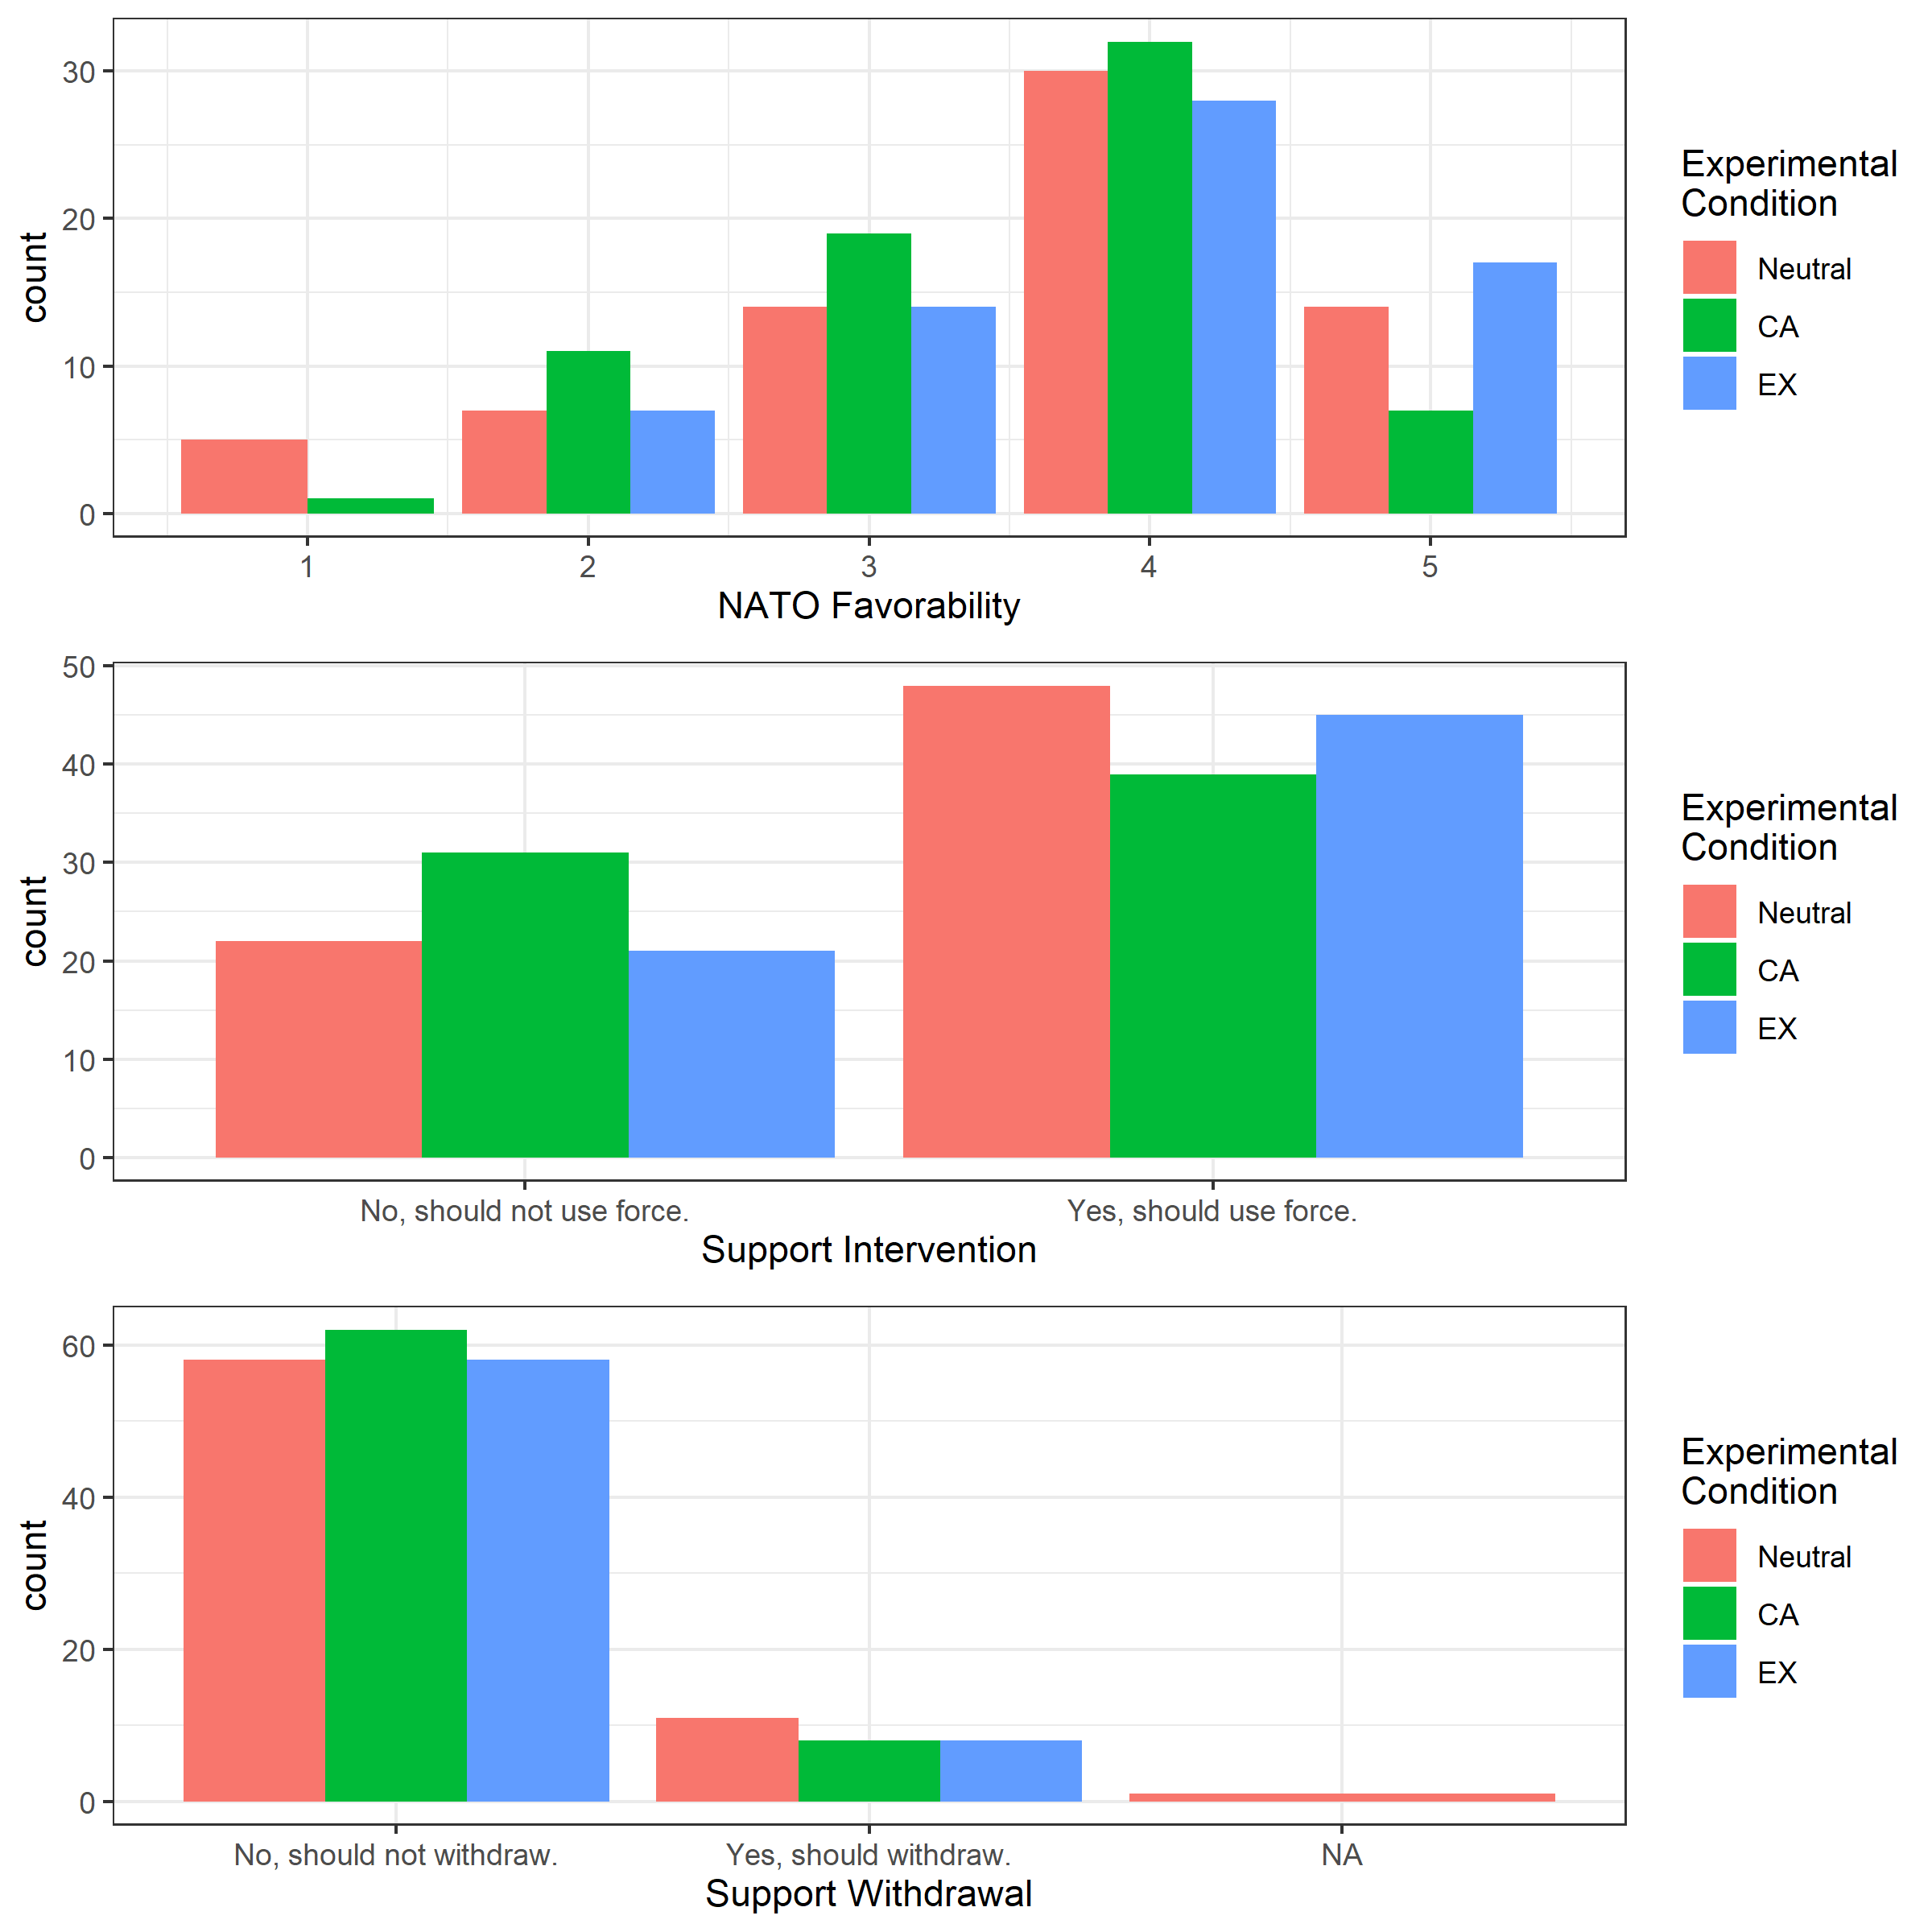
\includegraphics[width = .95\textwidth]{../figures/raw-data.png} 
\caption{Distribution of responses across different treatments in survey experiment on views towards NATO in the United States. Sample recruited on Mechanical Turk.}
\label{fig:raw-us-data}
\end{figure}


There is little difference in support for intervention in a hypothetical conflict between Russia and a NATO member across the neutral and exchange frames- both have high support for intervention. 
Almost 70\% of respondents in these two frames are willing to use force on behalf of NATO. 
Support for intervention falls to 55\% under a collective action frame.\footnote{Information about the purpose of NATO as supporting other states in war may explain this finding.} 


Framing relative military spending has no effect on support for withdrawal. 
Support for withdrawal is roughly constant across groups, as it ranges from 12 to 15\%. 
Thus, framing of relative military spending by NATO members does not change U.S. attitudes towards withdrawal. 
As expected framing has a weaker effect on policy choices than favorability. 


Regression models that adjust for other factors make similar inferences- exchange frames slightly increase favorability, and collective action frames slightly decrease support for military intervention. 
I summarize the treatment and control variable estimates in \autoref{fig:mturk-res-both}.
The positive estimate for exchange framing on favorability is statistically significant at the 5\% level in a one-tailed test. 
The negative estimate for collective action framing and military intervention is statistically significant at the 10\% level in a one-tailed test.
Therefore, the collective action and exchange frames have weak or null effects on attitudes towards NATO in the United States. 


\begin{figure}
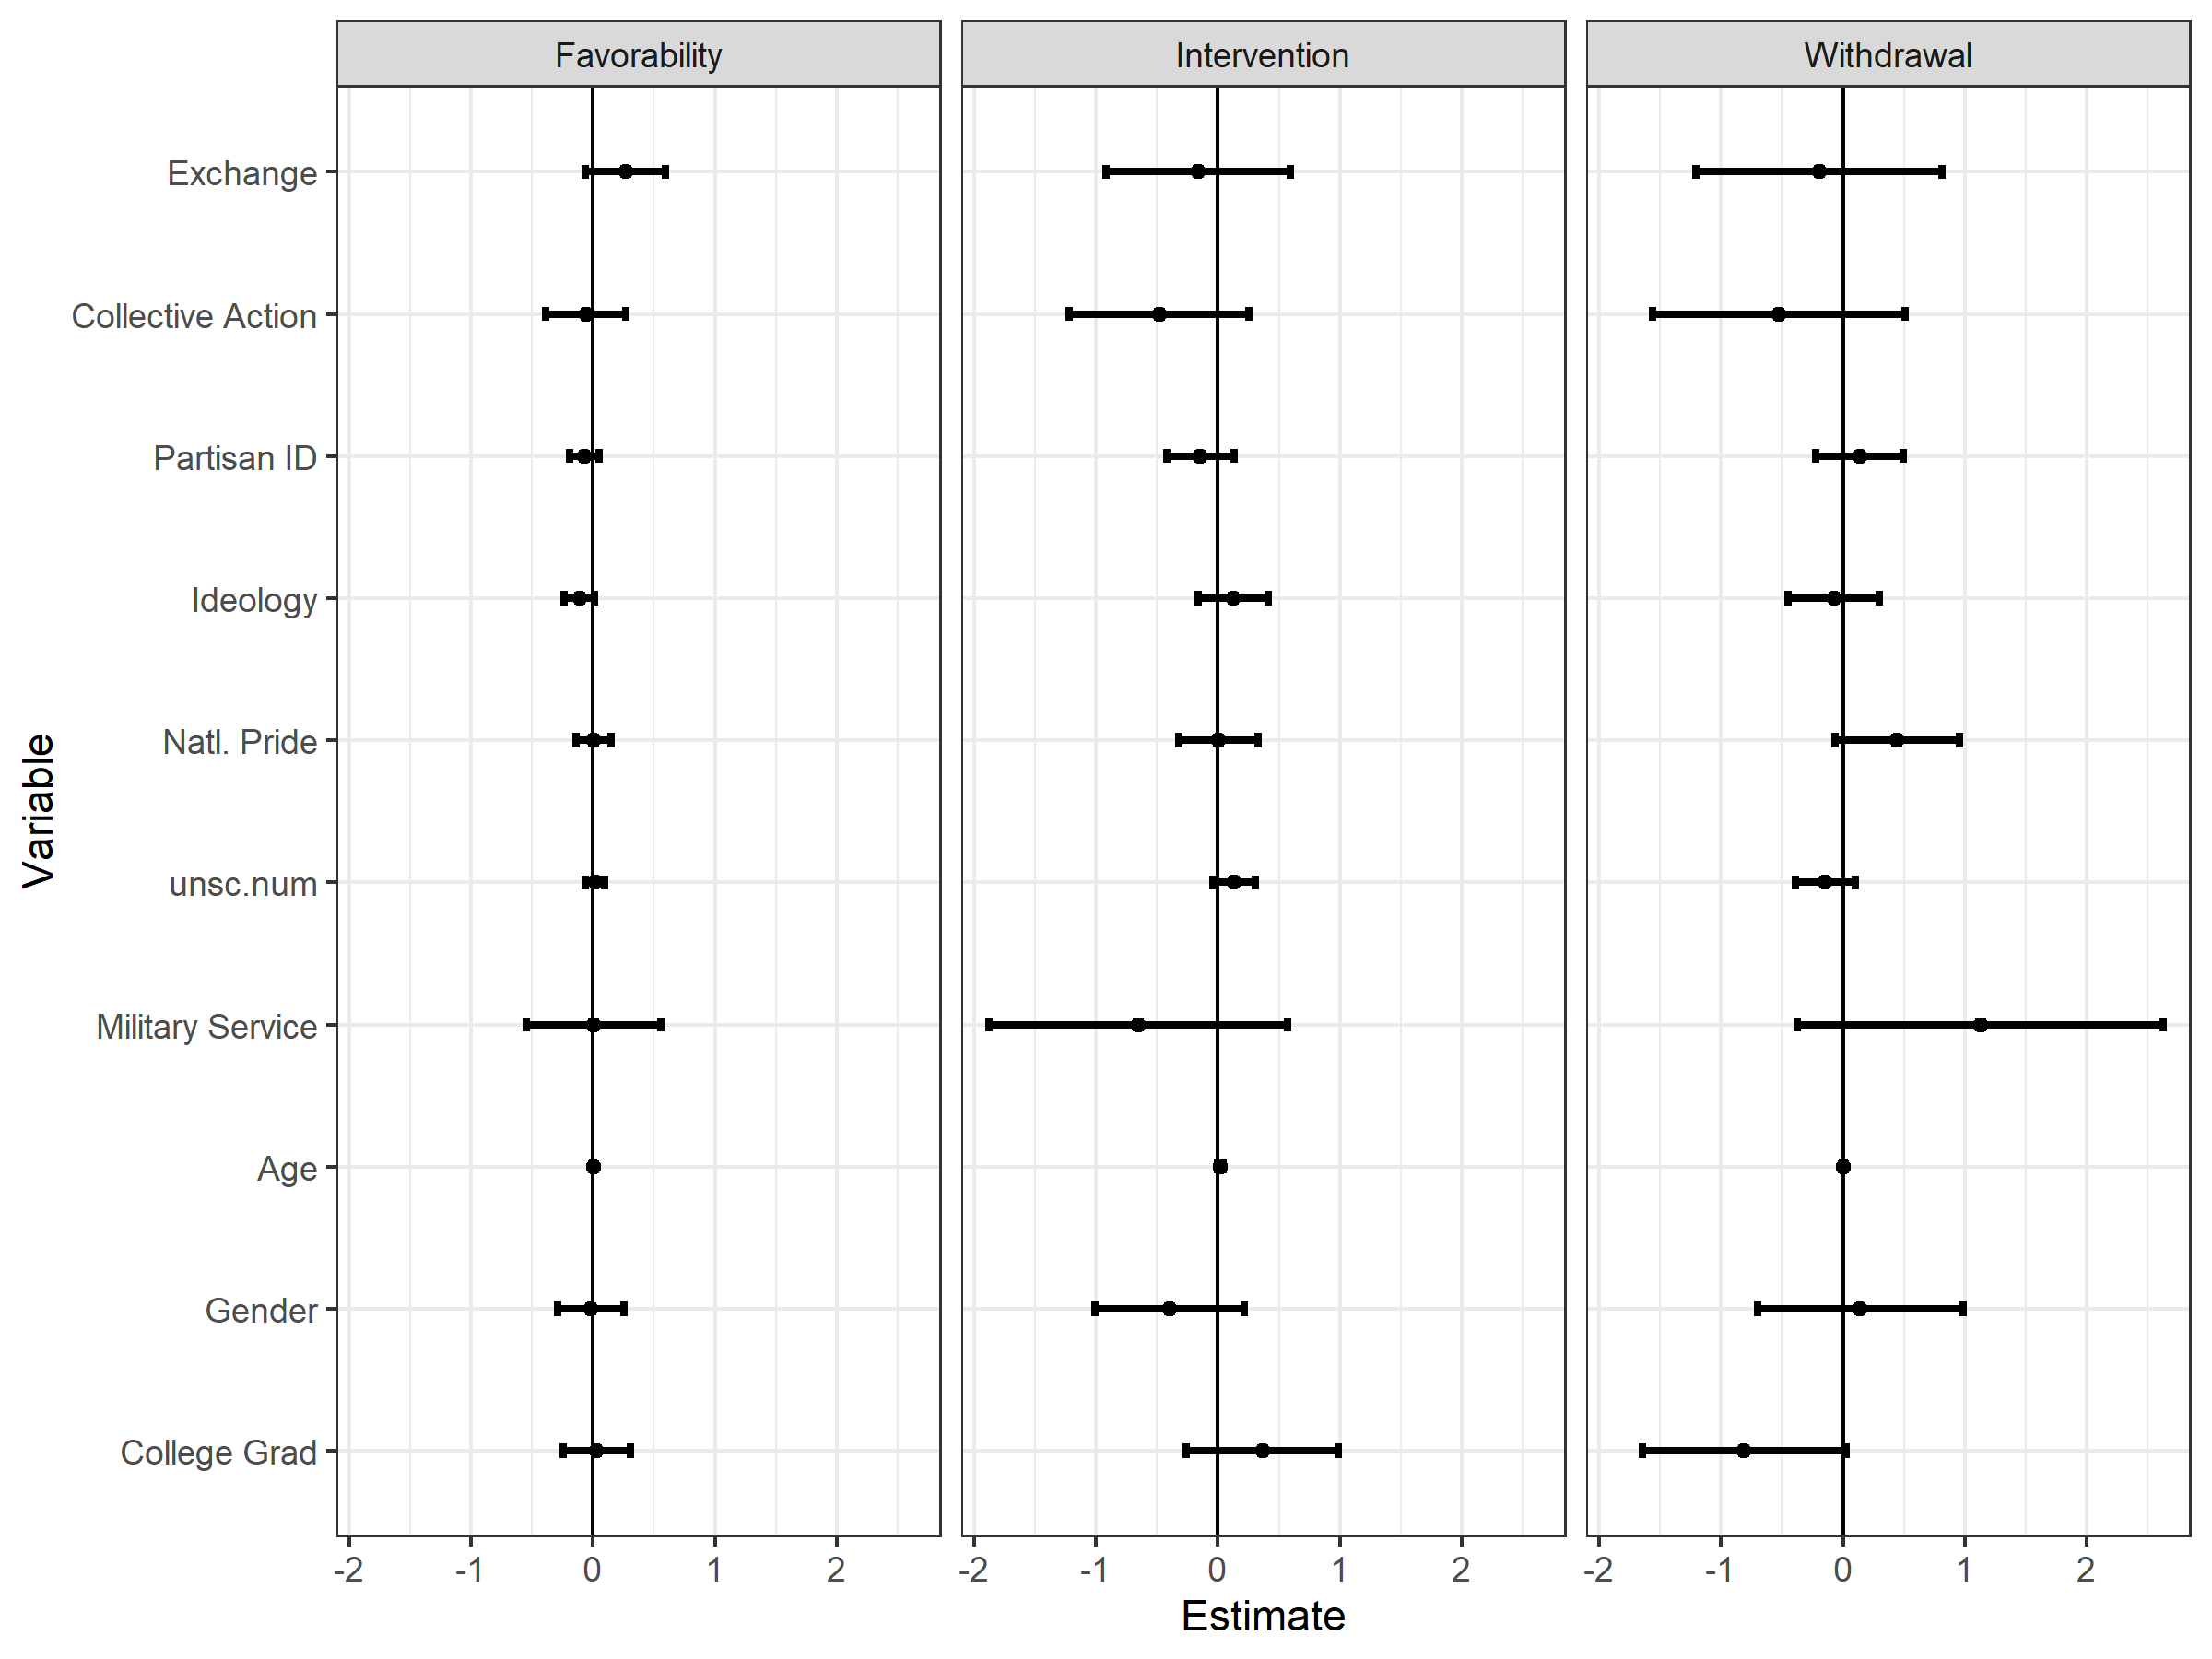
\includegraphics[width = .95\textwidth]{../figures/mturk-res-both.png} 
\caption{Estimated treatment effects and association between control variables with favorability towards NATO, support for intervention in conflict, and withdrawal from NATO. Data from Mechanical Turk.}
\label{fig:mturk-res-both}
\end{figure}


% discuss the results: conditional relationships, MTurk sample, weak frames, etc. 
There are several potential explanations for the weak relationship between the frames and attitudes towards NATO, which include design issues, conditional relationships and Mechanical Turk sample concerns.  
First, the power calculations behind 70 respondents in each group assumed an effect of roughly .75, so the study may not have enough power to detect smaller effects.
Second, the experimental frames may be too weak. 
While both frames lay out clear advantages and disadvantages, they also mention the role of military support in NATO. 
Perhaps as a result, support for military intervention is 15 to 20 points higher in the neutral and exchange frames than survey results from the Pew Research Center, which find that roughly half of U.S. respondents support intervention. 
Thus, the next iteration of the study should employ a larger sample and remove the information about military support in NATO from the vignettes. 


% conditional relationships
This pre-test sample is also not large enough to reliably estimate conditional relationships. 
Estimating interactions requires a sample size roughly six times as large as necessary for estimating main effects. 
There are also multiple potential interactions between partisanship, education, and foreign policy information, which I highlight in the argument. 
The presence of two treatments further increases the difficulty of estimating interactions. 
To estimate multiple interactions, I used a multilevel model that partially pools interactions between the treatments and education, partisanship and foreign policy information.
This turns up little evidence of heterogeneous treatment effects.\footnote{Results on file with the author.}


% MTurk Sample: higher education, partisan split leans Democract , 
Last, a Mechanical Turk sample may not represent the U.S. population. 
The sample has a larger share of strong Democrats and college graduates than the population. 
An unusual share of respondents was able to identify all five members of the UN security council correctly as well. 
Thus, this sample is better informed and more liberal than the US population.
Given widespread coverage of Trump's alliance rhetoric, this group may be more likely to support NATO than others. 


In fact, one of the potential reasons collective action has no effect of favorability is that individuals have been ``pretreated'' with collective action rhetoric by elites in the media. 

\subsection{German Results} 



\section{Discussion and Conclusion} 



\newpage

% Bibliography
\singlespace
 
\bibliography{../../MasterBibliography} 




\end{document}
